\documentclass{standalone}
\usepackage{tikz}
\usetikzlibrary{patterns, positioning}
\usetikzlibrary{shapes.misc}
\usepackage[outline]{contour}
\contourlength{1.5pt} 


\begin{document}
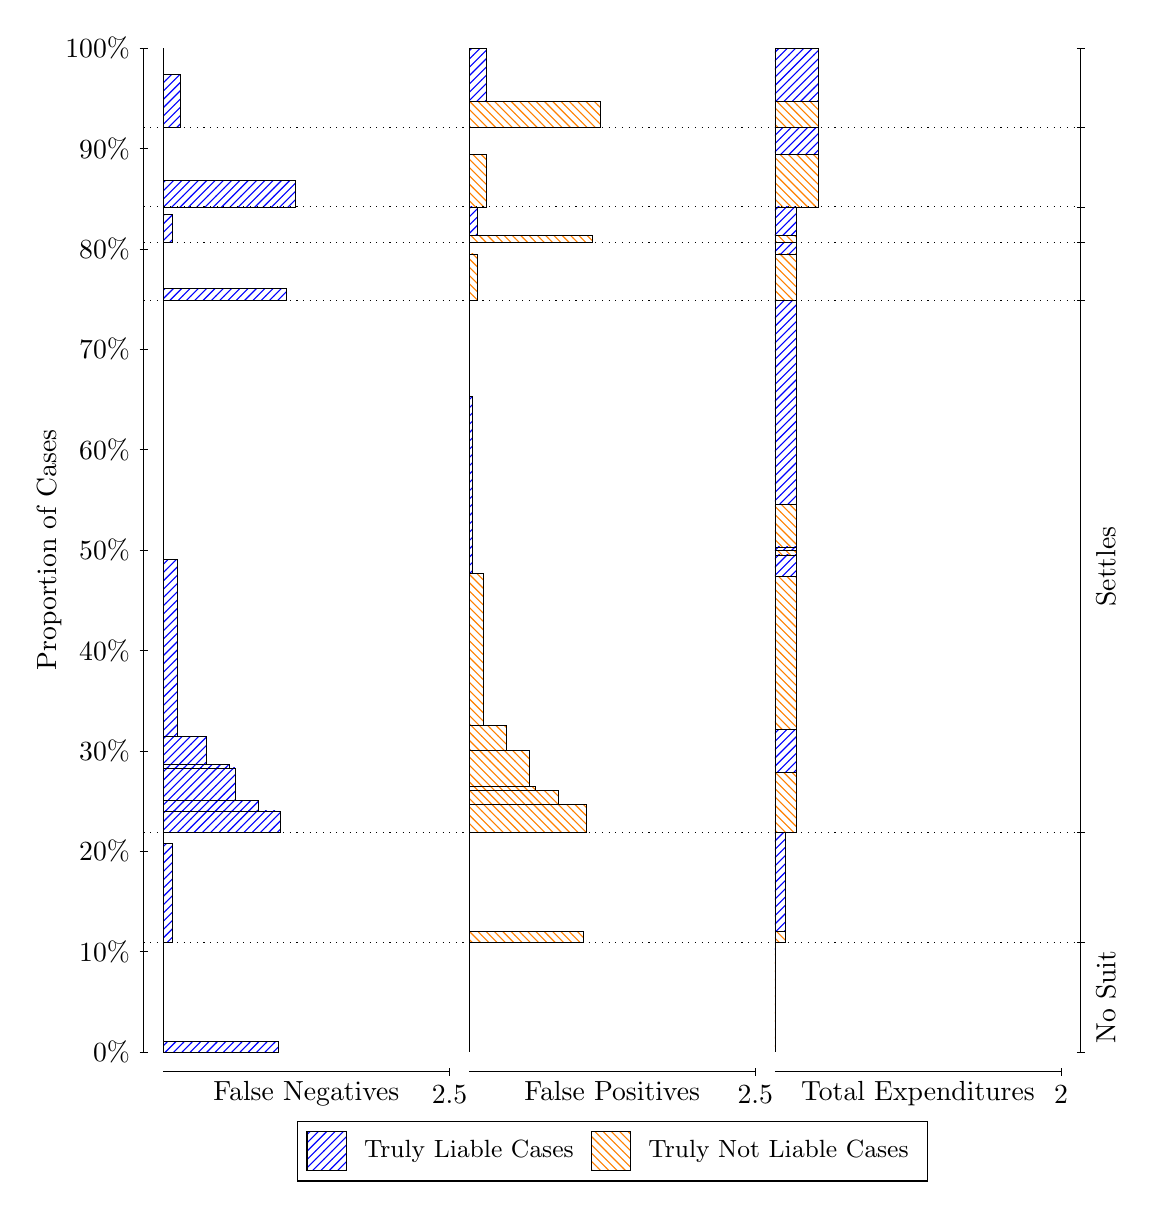
\begin{tikzpicture}
\draw[black, very thin] (1.5,1.75) -- (1.5,14.5);
\node[rotate=90, text=black, anchor=center] at (0.3, 8.125) {Proportion of Cases};
\draw[black, very thin] (1.45,1.75) -- (1.55,1.75);
\node[text=black, anchor=east] at (1.45, 1.75) {0\%};
\draw[black, very thin] (1.45,3.025) -- (1.55,3.025);
\node[text=black, anchor=east] at (1.45, 3.025) {10\%};
\draw[black, very thin] (1.45,4.3) -- (1.55,4.3);
\node[text=black, anchor=east] at (1.45, 4.3) {20\%};
\draw[black, very thin] (1.45,5.575) -- (1.55,5.575);
\node[text=black, anchor=east] at (1.45, 5.575) {30\%};
\draw[black, very thin] (1.45,6.85) -- (1.55,6.85);
\node[text=black, anchor=east] at (1.45, 6.85) {40\%};
\draw[black, very thin] (1.45,8.125) -- (1.55,8.125);
\node[text=black, anchor=east] at (1.45, 8.125) {50\%};
\draw[black, very thin] (1.45,9.4) -- (1.55,9.4);
\node[text=black, anchor=east] at (1.45, 9.4) {60\%};
\draw[black, very thin] (1.45,10.675) -- (1.55,10.675);
\node[text=black, anchor=east] at (1.45, 10.675) {70\%};
\draw[black, very thin] (1.45,11.95) -- (1.55,11.95);
\node[text=black, anchor=east] at (1.45, 11.95) {80\%};
\draw[black, very thin] (1.45,13.225) -- (1.55,13.225);
\node[text=black, anchor=east] at (1.45, 13.225) {90\%};
\draw[black, very thin] (1.45,14.5) -- (1.55,14.5);
\node[text=black, anchor=east] at (1.45, 14.5) {100\%};

\draw[black, very thin] (13.4,1.75) -- (13.4,14.5);
\draw[black, very thin] (13.35,1.75) -- (13.45,1.75);
\node[anchor=west] at (13.35, 1.75) {};
\draw[black, very thin] (13.35,3.1433) -- (13.45,3.1433);
\node[anchor=west] at (13.35, 3.1433) {};
\draw[black, very thin] (13.35,4.5357) -- (13.45,4.5357);
\node[anchor=west] at (13.35, 4.5357) {};
\draw[black, very thin] (13.35,11.298) -- (13.45,11.298);
\node[anchor=west] at (13.35, 11.298) {};
\draw[black, very thin] (13.35,12.031) -- (13.45,12.031);
\node[anchor=west] at (13.35, 12.031) {};
\draw[black, very thin] (13.35,12.483) -- (13.45,12.483);
\node[anchor=west] at (13.35, 12.483) {};
\draw[black, very thin] (13.35,13.488) -- (13.45,13.488);
\node[anchor=west] at (13.35, 13.488) {};
\draw[black, very thin] (13.35,14.5) -- (13.45,14.5);
\node[anchor=west] at (13.35, 14.5) {};

\draw[black, very thin, pattern color=blue, pattern=north east lines] (1.75,1.75) rectangle (3.2033,1.8849);
\draw[black, very thin, pattern color=orange, pattern=north west lines] (1.75,1.8849) rectangle (1.75,3.1433);
\draw[black, very thin, pattern color=blue, pattern=north east lines] (1.75,3.1433) rectangle (1.859,4.4013);
\draw[black, very thin, pattern color=orange, pattern=north west lines] (1.75,4.4013) rectangle (1.75,4.5357);
\draw[black, very thin, pattern color=blue, pattern=north east lines] (1.75,4.5357) rectangle (3.2397,4.812);
\draw[black, very thin, pattern color=blue, pattern=north east lines] (1.75,4.812) rectangle (2.949,4.9442);
\draw[black, very thin, pattern color=blue, pattern=north east lines] (1.75,4.9442) rectangle (2.6583,5.3587);
\draw[black, very thin, pattern color=blue, pattern=north east lines] (1.75,5.3587) rectangle (2.5857,5.4055);
\draw[black, very thin, pattern color=blue, pattern=north east lines] (1.75,5.4055) rectangle (2.295,5.7582);
\draw[black, very thin, pattern color=blue, pattern=north east lines] (1.75,5.7582) rectangle (1.9317,8.0022);
\draw[black, very thin, pattern color=orange, pattern=north west lines] (1.75,8.0022) rectangle (1.75,11.298);
\draw[black, very thin, pattern color=blue, pattern=north east lines] (1.75,11.298) rectangle (3.3123,11.443);
\draw[black, very thin, pattern color=orange, pattern=north west lines] (1.75,11.443) rectangle (1.75,12.031);
\draw[black, very thin, pattern color=blue, pattern=north east lines] (1.75,12.031) rectangle (1.859,12.39);
\draw[black, very thin, pattern color=orange, pattern=north west lines] (1.75,12.39) rectangle (1.75,12.483);
\draw[black, very thin, pattern color=blue, pattern=north east lines] (1.75,12.483) rectangle (3.4213,12.818);
\draw[black, very thin, pattern color=orange, pattern=north west lines] (1.75,12.818) rectangle (1.75,13.488);
\draw[black, very thin, pattern color=blue, pattern=north east lines] (1.75,13.488) rectangle (1.968,14.164);
\draw[black, very thin, pattern color=orange, pattern=north west lines] (1.75,14.164) rectangle (1.75,14.5);
\draw[black, very thin, pattern color=orange, pattern=north west lines] (5.6333,1.75) rectangle (5.6333,3.0084);
\draw[black, very thin, pattern color=blue, pattern=north east lines] (5.6333,3.0084) rectangle (5.6333,3.1433);
\draw[black, very thin, pattern color=orange, pattern=north west lines] (5.6333,3.1433) rectangle (7.0867,3.2778);
\draw[black, very thin, pattern color=blue, pattern=north east lines] (5.6333,3.2778) rectangle (5.6333,4.5357);
\draw[black, very thin, pattern color=orange, pattern=north west lines] (5.6333,4.5357) rectangle (7.123,4.8963);
\draw[black, very thin, pattern color=orange, pattern=north west lines] (5.6333,4.8963) rectangle (6.7597,5.0738);
\draw[black, very thin, pattern color=orange, pattern=north west lines] (5.6333,5.0738) rectangle (6.469,5.1275);
\draw[black, very thin, pattern color=orange, pattern=north west lines] (5.6333,5.1275) rectangle (6.3963,5.5776);
\draw[black, very thin, pattern color=orange, pattern=north west lines] (5.6333,5.5776) rectangle (6.1057,5.8951);
\draw[black, very thin, pattern color=orange, pattern=north west lines] (5.6333,5.8951) rectangle (5.815,7.8317);
\draw[black, very thin, pattern color=blue, pattern=north east lines] (5.6333,7.8317) rectangle (5.6697,10.076);
\draw[black, very thin, pattern color=blue, pattern=north east lines] (5.6333,10.076) rectangle (5.6333,11.298);
\draw[black, very thin, pattern color=orange, pattern=north west lines] (5.6333,11.298) rectangle (5.7423,11.885);
\draw[black, very thin, pattern color=blue, pattern=north east lines] (5.6333,11.885) rectangle (5.6333,12.031);
\draw[black, very thin, pattern color=orange, pattern=north west lines] (5.6333,12.031) rectangle (7.1957,12.124);
\draw[black, very thin, pattern color=blue, pattern=north east lines] (5.6333,12.124) rectangle (5.7423,12.483);
\draw[black, very thin, pattern color=orange, pattern=north west lines] (5.6333,12.483) rectangle (5.8513,13.153);
\draw[black, very thin, pattern color=blue, pattern=north east lines] (5.6333,13.153) rectangle (5.6333,13.488);
\draw[black, very thin, pattern color=orange, pattern=north west lines] (5.6333,13.488) rectangle (7.3047,13.824);
\draw[black, very thin, pattern color=blue, pattern=north east lines] (5.6333,13.824) rectangle (5.8513,14.5);
\draw[black, very thin, pattern color=orange, pattern=north west lines] (9.5167,1.75) rectangle (9.5167,3.0084);
\draw[black, very thin, pattern color=blue, pattern=north east lines] (9.5167,3.0084) rectangle (9.5167,3.1433);
\draw[black, very thin, pattern color=orange, pattern=north west lines] (9.5167,3.1433) rectangle (9.6529,3.2778);
\draw[black, very thin, pattern color=blue, pattern=north east lines] (9.5167,3.2778) rectangle (9.6529,4.5357);
\draw[black, very thin, pattern color=orange, pattern=north west lines] (9.5167,4.5357) rectangle (9.7892,5.3033);
\draw[black, very thin, pattern color=blue, pattern=north east lines] (9.5167,5.3033) rectangle (9.7892,5.85);
\draw[black, very thin, pattern color=orange, pattern=north west lines] (9.5167,5.85) rectangle (9.7892,7.7867);
\draw[black, very thin, pattern color=blue, pattern=north east lines] (9.5167,7.7867) rectangle (9.7892,8.0629);
\draw[black, very thin, pattern color=orange, pattern=north west lines] (9.5167,8.0629) rectangle (9.7892,8.1166);
\draw[black, very thin, pattern color=blue, pattern=north east lines] (9.5167,8.1166) rectangle (9.7892,8.1634);
\draw[black, very thin, pattern color=orange, pattern=north west lines] (9.5167,8.1634) rectangle (9.7892,8.7015);
\draw[black, very thin, pattern color=blue, pattern=north east lines] (9.5167,8.7015) rectangle (9.7892,11.298);
\draw[black, very thin, pattern color=orange, pattern=north west lines] (9.5167,11.298) rectangle (9.7892,11.885);
\draw[black, very thin, pattern color=blue, pattern=north east lines] (9.5167,11.885) rectangle (9.7892,12.031);
\draw[black, very thin, pattern color=orange, pattern=north west lines] (9.5167,12.031) rectangle (9.7892,12.124);
\draw[black, very thin, pattern color=blue, pattern=north east lines] (9.5167,12.124) rectangle (9.7892,12.483);
\draw[black, very thin, pattern color=orange, pattern=north west lines] (9.5167,12.483) rectangle (10.062,13.153);
\draw[black, very thin, pattern color=blue, pattern=north east lines] (9.5167,13.153) rectangle (10.062,13.488);
\draw[black, very thin, pattern color=orange, pattern=north west lines] (9.5167,13.488) rectangle (10.062,13.824);
\draw[black, very thin, pattern color=blue, pattern=north east lines] (9.5167,13.824) rectangle (10.062,14.5);
\draw[black, dotted] (1.5,3.1433) -- (13.4,3.1433);
\draw[black, dotted] (1.5,4.5357) -- (13.4,4.5357);
\draw[black, dotted] (1.5,11.298) -- (13.4,11.298);
\draw[black, dotted] (1.5,12.031) -- (13.4,12.031);
\draw[black, dotted] (1.5,12.483) -- (13.4,12.483);
\draw[black, dotted] (1.5,13.488) -- (13.4,13.488);
\draw[black, very thin] (1.75,1.5) -- (5.3833,1.5);
\node[text=black, anchor=north] at (3.5667, 1.5) {False Negatives};
\draw[black, very thin] (5.3833,1.45) -- (5.3833,1.55);
\node[text=black, anchor=north] at (5.3833, 1.45) {2.5};

\draw[black, very thin] (5.6333,1.5) -- (9.2667,1.5);
\node[text=black, anchor=north] at (7.45, 1.5) {False Positives};
\draw[black, very thin] (9.2667,1.45) -- (9.2667,1.55);
\node[text=black, anchor=north] at (9.2667, 1.45) {2.5};

\draw[black, very thin] (9.5167,1.5) -- (13.15,1.5);
\node[text=black, anchor=north] at (11.333, 1.5) {Total Expenditures};
\draw[black, very thin] (13.15,1.45) -- (13.15,1.55);
\node[text=black, anchor=north] at (13.15, 1.45) {2};

\node[text=black, centered, rotate=90] at (13.72, 2.4467) {\contour{white}{No Suit}};

\node[text=black, centered, rotate=90] at (13.72, 7.917) {\contour{white}{Settles}};





\draw (7.449999999999999,1.5) node[draw=none] (baseCoordinate) {};
\begin{scope}[align=center]
        \matrix[scale=0.5, draw=black, below=0.5cm of baseCoordinate, nodes={draw}, column sep=0.1cm]{
            \node[rectangle, draw, minimum width=0.5cm, minimum height=0.5cm, pattern color=blue, pattern=north east lines] {}; &
            \node[draw=none, font=\small, text=black] (B) {Truly Liable Cases}; &
            \node[rectangle, draw, minimum width=0.5cm, minimum height=0.5cm, pattern color=orange, pattern=north west lines] {}; &
            \node[draw=none, font=\small, text=black] (B) {Truly Not Liable Cases}; \\
            };
\end{scope}

\end{tikzpicture}
\end{document}